\documentclass[10pt]{article}
\usepackage{preamble}

\def\FS{Formelsammlung}
\def\Fach{Felder, Wellen und Leitungen}
\title{\FS \\ \Fach}
\date{\today}
\def\Semester{Wintersemester 23/24}
\IfFileExists{info.tex}
{
   \input{info.tex}
}
{
   \author{\href{https://www.youtube.com/watch?v=yMR45cZbvDw}{Die Prinzen - Alles nur geklaut}}
   \def\MatNr{MATNR}
}

\begin{document}

\pagenumbering{gobble}
\begin{titlepage}
	\thispagestyle{empty}

	\begin{center}
		\includegraphics[width=0.7\textwidth]{../OTHR_OTHR_Logo}\\
		\vspace*{\stretch{1}}
		\Huge
		\textsc{\MyTitle}\\
		\vspace*{\stretch{0.25}}
		\large
		\textbf{\Semester}\\
		{\small
		nach Vorlesung von Prof. Stücke und Prof. Sattler}

		\vspace*{\stretch{0.5}}
    Erstellt von\\ Max Forstner, \href{https://ayhamcloud.de/}{Ayham
    Alhulaibi}, \href{https://github.com/Vibeskanzler}{Tony Pham}  und Johannes
    Rothe\\


		\vspace*{\stretch{2}}
		{\renewcommand{\arraystretch}{1.5}
			\begin{tabular}{l l}
				Name:            & \hspace{4cm}\MyAuthor \\
				Matrikelnummer:  & \hspace{4cm}\MatNr    \\
				Letzte Änderung: & \hspace{4cm}\MyDate   \\
				Lizenz:          & \hspace{4cm}GPLv3
			\end{tabular}
		}
		\vspace*{\stretch{1}}
		\vspace*{\stretch{2}}


	\end{center}
\end{titlepage}

\newpage
\tableofcontents
\clearpage

\pagestyle{fancy}
\lhead{\MyAuthor}
\rhead{\Semester}
\cfoot{\vspace{-20pt}\thepage}
\pagenumbering{arabic}
% \setlength{\columnsep}{1pt}
\raggedcolumns

\begin{multicols*}{2}
	\input{sections/Grundlagen}
\end{multicols*}

% newpage
\include{sections/KoordinatenSysteme}
\section{Maxwell-Gleichungen}
\begin{table}[H]
	\centering
	\begin{tabularx}{\textwidth}{l | X | X}
		\makecell[l]{\textbf{Gaußsches Gesetz}} & 
			\(\boxed{\opdiv \vec{D} = \nabla \cdot \vec{D} = \rho}\) \par \vspace*{3pt} \footnotesize 
				Das elektrische Feld ist ein Quellenfeld. Die Ladung \(Q\) bzw. die Ladungsdichte \(\rho\) sind Quellen des elektrischen Feldes. & 
			\(\boxed{\oiint_{\partial V} \vec{D} \cdot \mathrm{d} \vec{a} = \iiint_V \rho \mathrm{d}V = Q}\) \par \vspace*{3pt} \footnotesize
				Der (elektrische) Fluss durch die geschlossene Oberfläche \(\partial V\) eines Volumens \(V\) ist gleich der elektrischen Ladung in seinem Inneren. \\
		\makecell[l]{\textbf{Gaußsches Gesetz} \\ \textbf{für Magnetismus}} & 
			\(\boxed{\opdiv \vec{B} = \nabla \cdot \vec{B} = 0}\) \par \vspace*{3pt} \footnotesize 
				Das magnetische Feld ist quellenfrei. Es gibt keine magnetischen Monopole. & 
			\(\boxed{\oiint_{\partial V} \vec{B} \cdot \mathrm{d} \vec{a} = 0}\) \par \vspace*{3pt} \footnotesize 
				Der mag. Fluss durch die geschlossene Oberfläche \(\partial V\) eines Volumens \(V\) entspricht der mag. Ladung in seinem Inneren, nämlich 0, da es keine magnetischen Monopole gibt. \\
		\makecell[l]{\textbf{Induktionsgesetz}} & 
			\(\boxed{\oprot \vec{E} = \nabla \times \vec{E} = -\frac{\partial \vec{B}}{\partial t}}\) \par \vspace*{3pt} \footnotesize 
				Jede zeitliche Änderung eines Magnetfeldes bewirkt ein elektrisches Wirbelfeld. & 
			\(\boxed{\oint_{\partial A} \vec{E} \cdot \mathrm{d} \vec{s} = -\iint_A \frac{\partial \vec{B}}{\partial t} \cdot \mathrm{d} \vec{a} = -\frac{\partial \Phi_{eingesch.}}{\partial t}}\)  \par \vspace*{3pt} \footnotesize 
				Die induzierte Umlaufspannung bzgl. der Randkurve \(\partial A\) einer Fläche \(A\) ist gleich der negativen zeitlichen Änderung des magnetischen Flusses durch diese Fläche. \\
		\makecell[l]{\textbf{Amperesches Gesetz} \\ \textbf{Durchflutungsgesetz}} & 
			\(\boxed{\oprot \vec{H} = \nabla \times \vec{H} = \vec{j} + \frac{\partial \vec{D}}{\partial t}}\) \par \vspace*{3pt} \footnotesize 
				Jeder Strom und jede zeitliche Änderung des elektrischen Feldes (Verschiebungsstrom) bewirkt ein magnetisches Wirbelfeld & 
			\(\boxed{\oint_{\partial A} \vec{H} \cdot \mathrm{d} \vec{s} = \iint_A \left( \vec{j} + \frac{\partial \vec{D}}{\partial t} \right) \cdot \mathrm{d} \vec{a}}\)  \par \vspace*{3pt} \footnotesize 
				Die mag. Umlaufspannung bzgl. der Randkurve \(\partial A\) einer Fläche \(A\) entspricht dem von dieser Fläche eingeschlossenen Strom (inkl. Verschiebungsstrom).
	\end{tabularx}
\end{table}

\subsection{Materialgleichungen}
	\begin{table}[H]
		\centering
		\begin{tabular}{l  l  l}
			\textbf{Differentielles ohmsches Gesetz} & \textbf{Materialgleichung} & \textbf{Materialgleichung} \\
			\(\boxed{\vec{J} = \kappa \cdot \vec{E} = \left[\frac{\mathrm{A}}{\mathrm{m}^2}\right]}\) & 
			\(\boxed{\vec{D} = \varepsilon \cdot \vec{E} = \left[\frac{\mathrm{C}}{\mathrm{m}^2}\right]}\) & 
			\(\boxed{\vec{B} = \mu \cdot \vec{H} = \left[\mathrm{T}\right]}\)
		\end{tabular}
	\end{table}

\subsection{Feldstärkekomponenten einer ebenen Welle}
	Bei Ausbreitung in $z$-Richtung gibt es keine Amplitudenabhängigkeit von $x, y$
	d.h. $\frac{\partial \ldots}{\partial x}=\frac{\partial \ldots}{\partial y}=0$ \\
	Ableitung einer harmonischen Größe nach der Zeit ergibt $\frac{\partial \ldots}{\partial t}=\mathrm{j} \omega \ldots$ 

	damit ergibt sich aus den Maxwell'schen Gleichungen:
	{\footnotesize
	$$
		\begin{gathered}
			\boxed{\operatorname{rot} \underline{\vec{E}}=-\mathrm{j} \omega \mu \underline{\vec{H}}} \qquad \boxed{\operatorname{rot} \underline{\vec{H}}=\mathrm{j} \omega \varepsilon \underline{\vec{E}}} \\
			\operatorname{rot} \underline{\vec{E}}=\left|\begin{array}{ccc}
				\vec{e}_x                   & \vec{e}_y                   & \vec{e}_z                   \\
				\frac{\partial}{\partial x} & \frac{\partial}{\partial y} & \frac{\partial}{\partial z} \\
				\underline{E}_x             & \underline{E}_y             & \underline{E}_z
			\end{array}\right|=\left(\begin{array}{c}
					\frac{\partial \underline{E}_z}{\partial y}-\frac{\partial \underline{E}_y}{\partial z} \\
					\frac{\partial \underline{E}_x}{\partial z}-\frac{\partial \underline{E}_z}{\partial x} \\
					\frac{\partial \underline{E}_y}{\partial x}-\frac{\partial \underline{E}_x}{\partial y}
				\end{array}\right)=\left(\begin{array}{l}
					0-\frac{\partial \underline{E}_y}{\partial z} \\
					\frac{\partial \underline{E}_x}{\partial z}-0 \\
					0-0
				\end{array}\right)=-\mathrm{j} \omega \mu\left(\begin{array}{l}
					\underline{H}_x \\
					\underline{H}_y \\
					\underline{H}_z
				\end{array}\right) \\
			\operatorname{rot} \underline{\vec{H}}=\left|\begin{array}{ccc}
				\vec{e}_x                   & \vec{e}_y                   & \vec{e}_z                   \\
				\frac{\partial}{\partial x} & \frac{\partial}{\partial y} & \frac{\partial}{\partial z} \\
				\underline{H}_x             & \underline{H}_y             & \underline{H}_z
			\end{array}\right|=\left(\begin{array}{c}
					\frac{\partial \underline{H_z}}{\partial y}-\frac{\partial \underline{H}_y}{\partial z} \\
					\frac{\partial \underline{H}_x}{\partial z}-\frac{\partial \underline{H}_z}{\partial x} \\
					\frac{\partial \underline{H}_y}{\partial x}-\frac{\partial \underline{H}_x}{\partial y}
				\end{array}\right)=\left(\begin{array}{c}
					0-\frac{\partial \underline{H}_y}{\partial z} \\
					\frac{\partial \underline{H}_x}{\partial z}-0 \\
					0-0
				\end{array}\right)=\mathrm{j} \omega \varepsilon\left(\begin{array}{l}
					\underline{E}_x \\
					\underline{E}_y \\
					\underline{E}_z
				\end{array}\right)
		\end{gathered}
	$$
	}

\subsection{Integralsätze}
	\begin{description}
		\setlength{\itemsep}{1pt}
		\item Fundamentalsatz der Analysis
		\item Gauß: Vektorfeld das aus Oberfläche von Volumen strömt muss aus Quelle in Volumen
		\item Stokes: innere Wirbel kompensieren sich $\rightarrow$ nur den Rand betrachten.
	\end{description}
	\begin{align*}
		\int_{a}^b \opgrad F \cdot d \vec{s}     & = F(b) - F(a)                                  \\
		\iiint_V \opdiv \vec{A} \cdot dV         & = \oiint_{ \partial V} \vec{A} \cdot d \vec{a} \\
		\iint_{A} \oprot \vec{A} \cdot d \vec{a} & = \oint_{ \partial A} \vec{A} \cdot d \vec{r}
	\end{align*}





\begin{multicols*}{2}
	\section{Felder}
\textbf{Feldunterscheidung}
\begin{align*}
	 & \vec{E}(x,y,z)                               & \widehat= & \quad\text{statisches Feld}  & \\
	 & \vec{E}(x,y,z,t)                             & \widehat= & \quad\text{quasi-stationäres Feld} & \\
	 & \vec{E}(x,y,z,t)\cdot cos(\omega t -\beta z) & \widehat= & \quad\text{Welle}            &
\end{align*}

\subsection{Elektrostatik}
	Wirbelfreie Felder $\rightarrow$ Gradientenfeld $\rightarrow$ elek. Ladungen
	sind Quellen des $\vec{E}$-Feldes (Skalare Potenzialfkt. $ \varphi $)
	\begin{align*}
		\oprot \vec{E} & = 0 = \oprot \opgrad \varphi & \vec{E} & = -\opgrad \varphi    & \\
		\opdiv \vec{D} & = \rho                 & \vec{D} & = \varepsilon \vec{E} &
	\end{align*}

	\subsubsection{Potential-/Poisson-Gleichung}
		La-Place-Gleichung, wenn $ \rho = 0 $

		\begin{align*}
			\opdiv \opgrad \varphi = \Delta \varphi & = - \dfrac{\rho}{\varepsilon}           \\
			\Delta \varphi + \underbrace{ \dfrac{\opgrad \varepsilon \cdot \opgrad \varphi}{\varepsilon}}_{= 0\texttt{, wenn homogen}}
													& = - \dfrac{\rho (x, y, z)}{\varepsilon}
		\end{align*}

		\textbf{meistens Ziel: Vereinfachung zu 1 Variable}

	\subsubsection{Randwertprobleme, -bedingungen (RB)}
		\textbf{Dirichlet-RB}: Gesuchte Potenzialfunktion $ \varphi $ nimmt an den
		Rändern einen bestimmten Wert an (Bsp.: $\rho_r = 5V$)

		\textbf{Neumann-RB}: Die Normalenableitung $ \tfrac{\partial\varphi}{\partial
				n} $ der Fkt. $ \varphi $ nimmt an den Rändern einen bestimmten Wert an. \\
		(Bsp.: Grenzfläche unterschiedlicher Dielektrika) \\
		\(\frac{\partial \varphi}{\partial n} = \opgrad \varphi \cdot \vec{n}\), \(\vec{n}\): Normalenvektor

	\subsubsection{Green'sche Funktionen}
		\textbullet{\textbf{Skalarpotential} einer Punktladung}
		\[ \varphi (r) = \dfrac{Q}{4 \pi \varepsilon_0 \cdot r} \qquad\left[V\right] \]

		\textbullet{\textbf{E-Feld} einer Punktladung}
		\[ \vec{E}(r) = \dfrac{Q}{4 \pi \varepsilon_0 \cdot r^2}\cdot\vec{e}_r \qquad\left[\frac{V}{m}\right] \]

		\textbullet{\textbf{D-Feld} einer Punktladung}
		\[ \vec{D}(r) = \dfrac{Q}{4 \pi \cdot r^2}\cdot\vec{e}_r \qquad\left[\frac{As}{m^2}=\frac{C}{m^2}\right] \]

		\textbullet{\textbf{Potentialfeld} einer Ladungsdichteverteilung}

		mit $\varphi(\infty)=0$
		\[
			\varphi(x, y, z)=\frac{1}{4 \pi \varepsilon} \iiint_{V^{\prime}}
			\frac{\rho\left(x^{\prime}, y^{\prime},
				z^{\prime}\right)}{\left|\vec{r}-\vec{r}^{\,\prime}\right|} \mathrm{d}
			V^{\prime}
		\]
		wobei:
		\begin{itemize}
			\item \(\vec{r}'\): Ortsvektor zum Punkt der Ladungsmenge
			\item \(\vec{r}\): Ortsvektor zum Aufpunkt \\ (Punkt, an dem das Potential berechnet werden soll)
		\end{itemize}

		mit der Green'schen Funktion $G\left(\vec{r},
			\vec{r}^{\,\prime}\right)=\frac{1}{4 \pi
				\varepsilon\left|\vec{r}-\vec{r}^{\,\prime}\right|}$
		\[ \varphi(x, y, z)=\iiint_{V^{\prime}} G\left(\vec{r}, \vec{r}^{\,\prime}\right) \rho\left(\vec{r}^{\,\prime}\right) \mathrm{d} V^{\prime} \]

		Vereinfachungen bei bekannter Ladungsverteilung:
		\begin{table}[H]
			\centering
			\begin{tabular}{l | c}
				Flächenladungsdichte \(\sigma\) & \(\varphi = \frac{1}{4\pi\epsilon} \iint_A' \frac{\sigma(x',y',z')}{\left|\vec{r} - \vec{r}'\right|} \mathsf{d}A'\) \\
				Linienladungsdichte \(\lambda\) & \(\varphi = \frac{1}{4\pi\epsilon} \int_s' \frac{\lambda(x',y',z')}{\left|\vec{r} - \vec{r}'\right|} \mathsf{d}s'\) \\
				Diskrete Punktladungen & \(\varphi = \frac{1}{4\pi\epsilon} \sum_{i=1}^N \frac{Q_i}{\left|\vec{r} - \vec{r}_i\right|}\)
			\end{tabular}
		\end{table}

	\subsubsection{Elektrischer Dipol}
		{\footnotesize Wird von Prof. Stücke nicht behandelt}
		\\
		Dipolmoment $\vec{p} = Q\cdot\vec{d}$

		\makebox[0pt][l]{
			\begin{minipage}[b]{0.5\columnwidth}
				\input{Figures/Felder/Elektrischer_Dipol_1.tex}
			\end{minipage}
			\begin{minipage}[b]{0.5\columnwidth}
				\input{Figures/Felder/Elektrischer_Dipol_2.tex}
			\end{minipage}
		}

		\makebox[0pt][l]{
			\begin{minipage}[]{0.5\columnwidth}
				\begin{align*}
					\varphi & = \frac{Q}{4\pi\varepsilon_0}\left(\frac{1}{r_1}-\frac{1}{r_2}\right)                                        \\
							& = \frac{Q}{4\pi\varepsilon_0}\cdot\frac{r_2-r_1}{r^2}                                                        \\
					\vec{E} & = -\nabla\varphi                                                                                             \\
							& = \frac{1}{4\pi\varepsilon_0}\cdot\left(\frac{3(\vec{p}\cdot\vec{r})\vec{r}}{r^5}-\frac{\vec{p}}{r^3}\right)
				\end{align*}
			\end{minipage}

			\begin{minipage}[]{0.5\columnwidth}
				\begin{align*}
					\varphi & \approx\frac{Qd\cos\theta}{4\pi\varepsilon_0r^2}                  \\
							& = \frac{1}{4\pi\varepsilon_0}\cdot\frac{\vec{p}\cdot\vec{r}}{r^3}
				\end{align*}
			\end{minipage}
		}

\subsection{Magnetostatik}
	Quellenfreie Wirbelfelder mit \textit{geschlossenen} Feldlinien.

	Keine magnetischen Monopole: $\opdiv \vec{B} = 0$.

	\begin{align*}
		\opdiv \vec{B} &= 0 = \opdiv \oprot \vec{A} & \oprot \vec{H} &= \vec{J} & \vec{B} &= \mu \vec{H} & \\
	\end{align*}

	\subsubsection{Vektorpotential}
		Reine Hilfsgröße, in Analogie zum elek. Skalarpotential $ \varphi $.

		\textbf{Coulomb-Eichung}, wenn $ \opdiv \vec{A} = 0 $, gilt \textbf{nur} für
		zeitunabhängige Felder.
		\begin{align*}
			\Delta \vec{A} & = - \mu \vec{J}  &
			\vec{B}        & = \oprot \vec{A} &
			\left[\vec{A} \right] = \frac{Wb}{m} = \frac{Vs}{m}
		\end{align*}

	\subsubsection{Vektorpotential in Abhängigkeit von der Stromdichte}
		\[
			\vec{A}(x, y, z)=\frac{\mu}{4 \pi} \iiint_{V^{\prime}} \frac{\vec{J}\left(x^{\prime}, y^{\prime}, z^{\prime}\right)}{\left|\vec{r}-\vec{r}^{\,\prime}\right|} d V^{\prime}
		\]

	\subsubsection{Biot-Savart-Gesetz}
		\[
			\vec{H}=\frac{I}{4 \pi} \oint_{C^{\prime}} \opgrad \frac{1}{\left|\vec{r}-\vec{r}^{\,\prime}\right|} \times \mathrm{d} \vec{s}^{\,\prime}
		\]

		mit $\opgrad \frac{1}{\left|\vec{r}-\vec{r}^{\,\prime}\right|}=-\frac{\vec{r}-\vec{r}^{\,\prime}}{\left|\vec{r}-\vec{r}^{\,\prime}\right|^{3}}$

		\[
			\vec{H}=\frac{I}{4 \pi} \oint_{C^{\prime}} \frac{\mathrm{d} \vec{s}^{\,\prime} \times\left(\vec{r}-\vec{r}^{\,\prime}\right)}{\left|\vec{r}-\vec{r}^{\,\prime}\right|^{3}}
		\]

		\begin{itemize}
			\footnotesize
			\item \(\vec{r}'\): Ortsvektor zum Punkt der Ladungsmenge
			\item \(\vec{r}\): Ortsvektor zum Aufpunkt \\ (Punkt, an dem das Magnetfeld berechnet werden soll)
		\end{itemize}

	\subsubsection{Magnetischer Dipol}
		{\footnotesize Wird von Prof. Stücke nicht behandelt}
		\input{Figures/Felder/Magnetischer_Dipol_1.tex}

		Strom $I$ entlang eines Leiters: $\left[\vec{A}\right] = \frac{Vs}{m}$
		\begin{flalign*}
			\vec{A}(r)                      & = \frac{\mu_0 \cdot I}{4 \pi} \int \frac{d \vec{R}}{| \vec{r} - \vec{R}|} = \frac{ \mu_0}{4 \pi} \frac{\vec{m} \times \vec{r}}{r^3} \\
			\vec{B} = \nabla \times \vec{A} & = \frac{\mu_0}{4 \pi} \left(\frac{3(\vec{m} \cdot \vec{r})\vec{r}}{r^5} - \frac{\vec{m}}{r^3}\right)
		\end{flalign*}

\subsection{Quasistationäre Felder (Wechselstrom)}
	Homogenes, Isotropes Medium: $ \varepsilon, \mu, \kappa = \mathtt{kost.} $\\
	Leiter ist quasineutral: $ \rho = 0 $. \(\frac{\partial}{\partial t} \ne 0 \quad \frac{\partial \vec{D}}{\partial t} \ll \vec{J}\)
	\begin{align*}
		\oprot \vec{E} & = -\frac{\partial \vec{B}}{\partial t} = -\mu \frac{\partial \vec{H}}{\partial t} & \opdiv \vec{E} & = 0 & \vec{D} & = \varepsilon\vec{E} & \\
		\oprot \vec{H} & = \vec{J} = \kappa \vec{E}                                                        & \opdiv \vec{B} & = 0 & \vec{B} & = \mu\vec{H}         & \\
		\opdiv \vec{J} & = -\frac{\partial \rho}{\partial t}                                               & \opdiv \vec{H} & = 0 & \vec{J} & = \kappa \vec{E}     &
	\end{align*}

	\subsubsection{Komplexe Feldgrößen}
	\textbullet komplexer Amplitudenvektor / Phasor:
	\begin{equation*}
		\underline{\vec{J}}=\vec{J}\cdot e^{j\varphi}
	\end{equation*}
	\textbullet komplexer Amplituden-Drehzeiger:
	\begin{align*}
		\underline{\vec{J}}(t) & =\underline{\vec{J}} \cdot e ^{j\omega t} = \vec{J} \cdot e^{j(\omega t+\varphi)}
	\end{align*}
	\textbullet Darstellung in karthesischen Koordinaten:
	\begin{align*}
		\underline{\vec{J}} & =\underline{J}_x \cdot \vec{e}_x + \underline{J}_y \cdot \vec{e}_y + \underline{J}_z \cdot \vec{e}_z
	\end{align*}

\subsection{Skineffekt}\label{sec:skineffekt}
	\begin{mdframed}[style=exercise]
		\begin{itemize}
			\item \textbf{Eindringtiefe}/Äquivalente Leitschichtdicke:\\
				\(\boxed{\delta = \frac{1}{\alpha} = \frac{1}{\beta} = \frac{1}{\sqrt{\pi\mu\kappa f}} = \sqrt{\frac{2}{\omega\mu\kappa}}} \quad \left[\delta\right] = m\)
			\item \textbf{Fortpflanzungskonstante: }\\
				\(\underline{\gamma} = \alpha + j \beta = \sqrt{\frac{\omega\mu\kappa}{2}} (1+j) \)
		\end{itemize}
	\end{mdframed}

	\subsubsection{unendlich breiter Leiter}
		\begin{figure}[H]
			\centering
			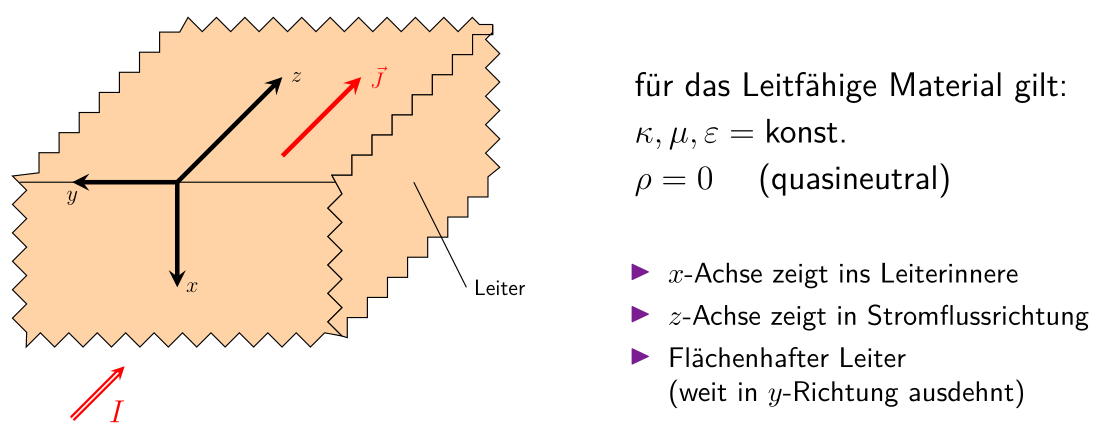
\includegraphics[width=0.9\columnwidth]{Figures/Felder/Skineffekt_unendlichBreit.png}
		\end{figure}
		Lösung durch DGL:
		\begin{align*}
			&\Delta \vec{\underline{E}} - j \omega \mu \kappa \vec{\underline{E}} = 0\\
			&\Delta \vec{\underline{H}} - j \omega \mu \kappa \vec{\underline{H}} = 0
		\end{align*}
		Annahme für Stromdichte:
		\begin{align*}
			\vec{\underline{J}} = \underline{J}_z \cdot \vec{e}_z \quad \text{mit } \vec{\underline{J}} = \kappa \vec{\underline{E}} \quad \vec{\underline{E}} = \underline{E}_z \cdot \vec{e}_z
		\end{align*}
		Lösung des Gleichungssystems ergibt:
		\begin{mdframed}[style=exercise]
			\begin{align*}
				\underline{E}_z(x,t) &= \underline{E}_0 e^{-\underline{\gamma}x} \cdot e^{j \omega t} = \underline{E}_0 e^{-\alpha x} e^{-j \beta x} \cdot e^{j \omega t} \\
				&= E_0 \cdot e^{- \alpha x} \cdot e^{j \left(\omega t - \beta x + \varphi_0\right)}\\
				\underline{H}_y(x,t) &= - \frac{\underline{\gamma}}{j \omega \mu} \underline{E}_z(x,t) = - \sqrt{\frac{\kappa}{\omega \mu}} e^{-j \frac{\pi}{4}} \cdot \underline{E}_z(x,t)\\
				&= - \sqrt{\frac{\kappa}{\omega \mu}} E_0 \cdot e^{- \alpha x} \cdot e^{j \left(\omega t - \beta x + \varphi_0 - \frac{\pi}{4}\right)}\\
			\end{align*}
		\end{mdframed}

	\subsubsection{Rundleiter}
		\input{Figures/Felder/Skineffekt.tex}

		\begin{description}
			\item (Oberflächen)\textbf{widerstand}:
				\begin{flalign*}
					R_{AC} & = \frac{l}{\kappa \cdot A_{\texttt{eff}}} &
					R_{DC} & =\dfrac{l}{\kappa \pi r_0^{2}}              &
					R_F    & = \dfrac{1}{\kappa \delta}                &
				\end{flalign*}

			\item \textbf{Feldstärke} verglichen mit der Oberfläche:\\
				Wenn \(\delta \ll r_0\), kann wie im unendlich breiten Leiter genähert werden mit e-Funktion. 
				Ansonsten keine genaue Aussage möglich (Bessel-Funktion). 

			\item \textbf{Rundleiter - Effektive Fläche}:
				% {\footnotesize
				% 	Gilt nur, wenn kleinste geometrische Abmessung \(> 10\delta\)
				% }
				\begin{align*}
					A_{\texttt{eff}} & = A_{\texttt{ges}} - A_{\sigma} = r_0^2\pi-(r_0-\delta)^2\pi = 2\cdot \pi \delta \left( r_0-\dfrac{\delta }{2}\right)
				\end{align*}
		\end{description}

	\subsubsection{Näherungen für Skineffekt im Rundleiter}
		\begin{figure}[H]
			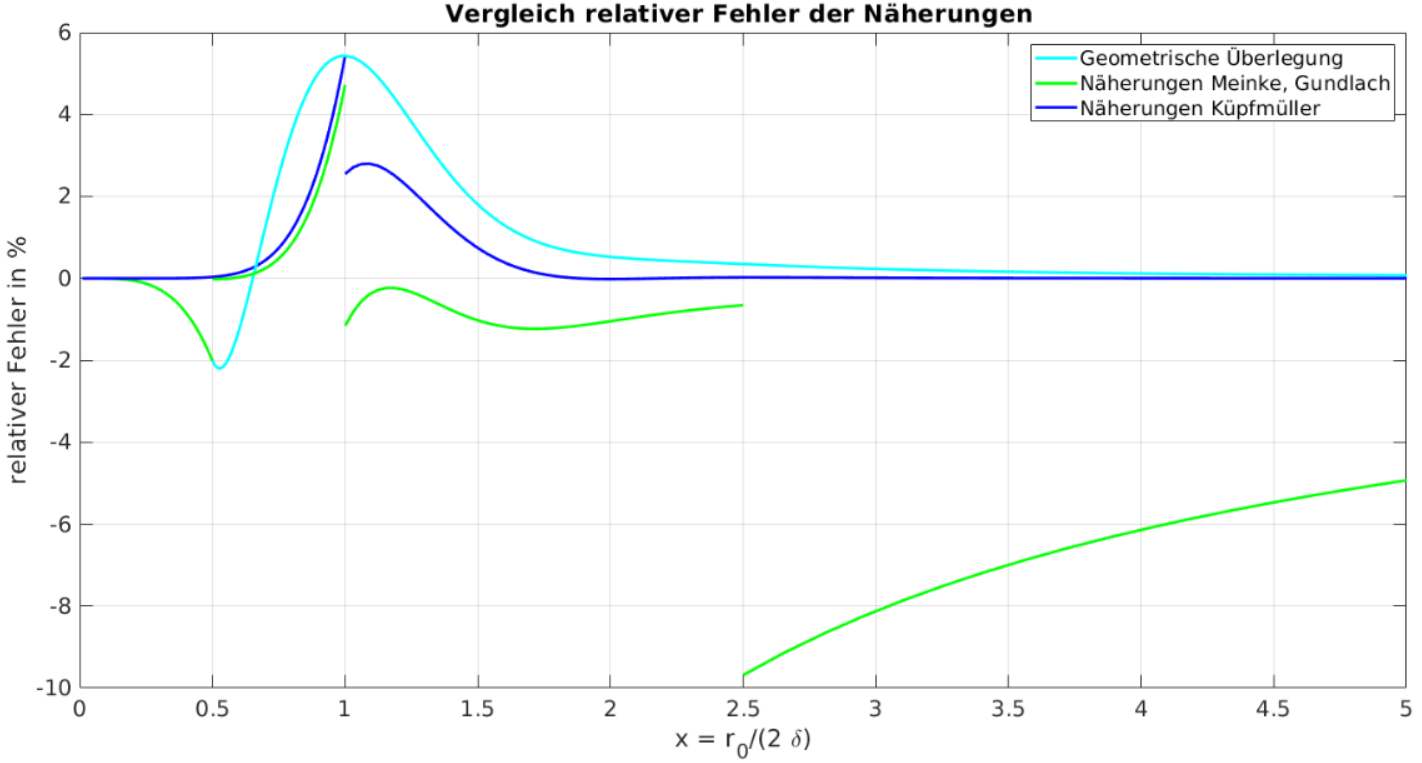
\includegraphics[width=0.98\columnwidth]{Figures/Felder/Skineffekt_Vergleich.png}
		\end{figure}
		\begin{description}
			\item \textbf{Geometrische} Beschreibung (Fehler $ < 6\% $)
				\begin{align*}
					\frac{R_{AC}}{R_{DC}} & =
					\begin{dcases}
						1                                                & \text{für} \quad r_0 < \delta    \\
						\frac{r_0^2}{2\cdot \delta \cdot r_0 - \delta^2} & \text{für} \quad r_0 \geq \delta
					\end{dcases}
				\end{align*}

			\item \textbf{Bessel}-Funktion (Fehler $ < 6 \% $) [Küpfmüller]:
				\begin{align*}
					\frac{R_{AC}}{R_{DC}} & =
					\begin{dcases}
						1 + \frac{1}{3}x^4              & \text{für} \qquad x < 1 \\
						x + \frac{1}{4} + \frac{3}{64x} & \text{für} \qquad x > 1 \\
					\end{dcases} \\
					\frac{X_{AC}}{R_{DC}} & =
					\begin{dcases}
						x^2\left( 1-\frac{x^4}{6} \right)   & \text{für} \qquad x < 1 \\
						x- \frac{3}{64x} + \frac{3}{128x^2} & \text{für} \qquad x > 1 \\
					\end{dcases}
				\end{align*}
				\[
					\boxed{x=\frac{r_0}{2\delta}} \qquad r_0 \, \hat{=} \textnormal{ Außenradius} \qquad X_{AC} = \omega L_i
				\]

			\item \textbf{Empirische} Beschreibung (Fehler $ < 10\% $) [Meinke, Gundlach]:
				\begin{align*}
					\frac{R_{AC}}{R_{DC}} & =
					\begin{dcases}
						1                                                & \text{für} \quad r_0 < \delta                      \\
						1+ \left( \frac{r_0}{2,65\cdot \delta} \right)^4 & \text{für} \quad \delta < r_0 < 2\delta            \\
						\frac{r_0}{2 \cdot\delta} + \frac{1}{4}          & \text{für} \quad 2\delta < r_0 < 5\delta \quad (1) \\
						\frac{r_0}{2\cdot \delta}                        & \text{für} \quad 5\delta < r_0 \quad (2)
					\end{dcases}
				\end{align*}
				\footnotesize Anmerkung: (1) $\widehat{=}$ Kreisring mit Näherung \quad
				(2) $\widehat{=}$ Ring mittig
		\end{description}

\subsection{E-Felder an Grenzflächen}
	\subsubsection{Dielektrische Grenzfläche}
		\textbf{Querschichtung}:
		\begin{align*}
			D_{1n} & = D_{2n} & \varepsilon_1 E_{1n} & =\varepsilon_2 E_{2n} &
		\end{align*}
		Schwächeres E-Feld bei höherem $ \varepsilon $.

		\vspace{0.5em}
		\textbf{Längsschichtung}:
		\begin{align*}
			E_{1t} & = E_{2t} & \frac{D_{1t}}{\varepsilon_1} & = \frac{D_{2t}}{\varepsilon_2} &
		\end{align*}

		Höheres D-Feld (mehr Ladungen) bei höherem $ \varepsilon $.

		\vspace{0.5em}
		\textbf{Schrägschichtung}:
		\begin{align*}
			& \frac{\tan( \alpha_1)}{\tan( \alpha_2)} = \frac{E_{1t}/E_{1n}}{E_{2t}/E_{2n}} = \frac{D_{2n}/\varepsilon_2}{D_{1n}/\varepsilon_1} = \frac{ \varepsilon_1}{\varepsilon_2}
		\end{align*}

	\subsubsection{Grenzfläche Dielektrikum-Leiter}
		Ladungen verschieben sich so lange, bis im Leiter kein Feld mehr herrscht.
		$\rightarrow E_{2t}, E_{2n}, D_{2t}, D_{2n} = 0 $

		\vspace{0.5em}
		\textbf{Längsschichtung}:
		\begin{align*}
			E_{1t} & = E_{2t} = 0 & D_{1t} & =\varepsilon_1 E_{1t} = 0 &
		\end{align*}
		Felder stehen stets senkrecht auf elek. Leitern.

		\vspace{0.5em}
		\textbf{Querschichtung}:
		\begin{align*}
			D_{1n} - D_{2n} & = \frac{Q}{A} & D_{1n} & = \frac{Q}{A} & E_{1n} & = \frac{Q}{\varepsilon_1 A} &
		\end{align*}

		D-Feld entspricht der Flächenladungsdichte des Leiters.

	\subsubsection{Grenzfläche an magn. Feldern}
		\textbf{Querschichtung}:
		\begin{align*}
			B_{1n} & = B_{2n} & \mu_1 H_{1n} & =\mu_2 H_{2n} &
		\end{align*}
		Schwächeres H-Feld bei höherem $ \mu $.\\

		\textbf{Längsschichtung}:
		\begin{align*}
			H_{1t} & = H_{2t} & \frac{B_{1t}}{\mu_1} & = \frac{B_{2t}}{\mu_2} &
		\end{align*}

		Höheres B-Feld (mehr Fluss) bei höherem $ \mu $.

		\vspace{0.5em}
		\textbf{Schrägschichtung}:
		\begin{align*}
			& \frac{\tan( \alpha_1)}{\tan( \alpha_2)} = \frac{ \mu_1}{\mu_2}
		\end{align*}

	\include{sections/Wellen}
	\include{sections/Leitungen}
	\include{sections/Wellenleiter}
	\include{sections/Smithdiagramm}
	\include{sections/Antennen}
\end{multicols*}
\include{sections/Antennentabelle}
\section{Einheiten} \label{sec:Einheiten}
\begin{tabular}{l|l|l}
    \hline
    Symbol & Größe & Einheit\\
    \hline 
    A, W & Arbeit, Energie & J = VAs = Ws\\
    $\vec{A}$ & mag. Vektorpotential & $\dfrac{Vs}{m} = \dfrac{Wb}{m}$ ($\vec{B}$ = $\nabla \times \vec{A}$)\\
    $\vec{B}$ & mag. Flussdichte & $T = \dfrac{Vs}{m^2}$\\
    C & Kapazität & $F = \dfrac{As}{V}$\\
    $\vec{D}$ & dielek. Verschiebung/Flussdichte & $\dfrac{As}{m^2} = \dfrac{C}{m^2}$\\
    e, q, Q & (Elementar-)ladung & C = As\\
    $\vec{E}$ & elek. Feldstärke & $\dfrac{V}{m}$ \\
    $\vec{H}$ & mag. Feldstärke/Erregung & $\dfrac{A}{m}$\\
    $\vec{J}$ & Stromdichte & $\dfrac{A}{m^2}$\\
    $\vec{J}_F$ & Flächenstromdichte & $\dfrac{A}{m}$\\
    $L$ & Induktivität & $\dfrac{kgm^2}{A^2s^2} = \dfrac{Wb}{A} = \Omega s$ \\
    $\vec{M}$ & Drehmoment & J = Nm = VAs\\
    F & Kraft & $\dfrac{kgm}{s^2} = N$\\
    $R_{mag}$ & mag. Widerstand & $\dfrac{1}{H} = \dfrac{A}{Vs}$\\
    $\vec{S}$ & Poynting-Vektor & $\dfrac{W}{m^2}$\\
    Z & Wellenwiderstand & $\Omega$\\
    $\delta_s$ & Eindringtiefe & m \\
    $\varepsilon$ & Dielektrizitätskonstante & $\dfrac{As}{Vm}$\\
    $\varphi$ & elek. Skalarpotential & V \\
    $\varphi_m$ & mag. Skalarpotential & A \\
    $\rho$ & Raumladungsdichte & $\dfrac{As}{m^3}$\\
    $\rho$ & spez. Widerstand & $\dfrac{\Omega mm^2}{m} = \dfrac{V \cdot mm^2}{A \cdot m}$\\
    $\kappa, \sigma$ & elek. Leitfähigkeit & $\dfrac{S}{m} = \dfrac{A}{Vm}$\\
    $\lambda$ & Wellenlänge & m\\
    $\mu$ & Permiabilitätskonstante & $\dfrac{Vs}{Am}$\\
    $\Phi_e$ & elek. Fluss & C = As\\
    $\Phi_m$ & mag. Fluss & $Wb = Vs = T \cdot m^2$\\

    \hline
\end{tabular}



\end{document}
